% !TEX program = xelatex
% Original Author: GitHub @leowrs (https://github.com/leowrs)
\documentclass[journal]{IEEEtran}
% Font Configuration
\usepackage{fontspec}
\setmainfont{Times New Roman}

% Packages
\usepackage{amsmath,amssymb,amsfonts}
\usepackage{graphicx}
\usepackage{cite}
\usepackage{booktabs}
\usepackage{multirow}
\usepackage{caption}
\usepackage{float}

% Title Info
\title{Evolution and Future of OFDM: A Comprehensive Survey on PAPR Reduction, Deep Learning, and ISAC Integration}

\author{@leowrs, \textit{School of Foreign Languages, Southeast University, Nanjing, China}\\
Email: https://github.com/leowrs}

\begin{document}

\maketitle

\begin{abstract}
    Orthogonal Frequency Division Multiplexing (OFDM) has cemented its role as the cornerstone of modern wireless communication systems, spanning from 4G LTE to 5G New Radio (NR) and IEEE 802.11be (Wi-Fi 7), driven by its spectral efficiency and robustness against multipath fading. However, the high Peak-to-Average Power Ratio (PAPR), inherent to multicarrier waveforms utilizing the Inverse Fast Fourier Transform (IFFT), remains a critical bottleneck. High PAPR forces High Power Amplifiers (HPA) to operate in their non-linear saturation region, causing severe spectral regrowth and in-band distortion, or necessitates operation with large Input Back-Offs (IBO), drastically reducing energy efficiency. While numerous surveys have cataloged classical reduction techniques like Selected Mapping (SLM) and Companding, they typically fail to address the paradigm shift introduced by data-driven approaches and emerging system architectures. Crucially, existing literature often lacks a unified framework connecting classical probabilistic methods with cutting-edge Deep Learning (DL) models. This paper bridges this gap by presenting a comprehensive taxonomy that integrates legacy algorithms with swarm intelligence and neural network-based optimizations. We provide a rigorous \textbf{Quantitative Trade-off Analysis}, contrasting the computational burden of iterative algorithms against their statistical CCDF gains using a unified metric. Furthermore, we extend the horizon to the 6G era, exploring PAPR reduction in the context of Non-Orthogonal Multiple Access (NOMA) and Integrated Sensing and Communication (ISAC), where waveforms must serve dual purposes. This survey aims to guide researchers through the evolution of OFDM, offering a roadmap from foundational theories to future intelligent, sensing-aware waveforms.
\end{abstract}

\begin{IEEEkeywords}
    OFDM, PAPR, Deep Learning, ISAC, 6G, SLM, PTS, Clipping.
\end{IEEEkeywords}

\section{Introduction}

\subsection{Historical Context and Motivation}
The concept of multicarrier modulation dates back to the seminal work by Weinstein and Ebert \cite{ref1} in 1971, which introduced the use of the Discrete Fourier Transform (DFT) to implement modulation and demodulation. Over the decades, OFDM has triumphed over competing technologies like CDMA (3G) to become the de facto standard for broadband communications. Its ability to equalize frequency-selective channels with a single-tap frequency-domain equalizer makes it indispensable for high-rate transmission.

However, the superposition of $N$ subcarriers with random phases results in a time-domain signal with a Rayleigh-distributed envelope, leading to occasional high peaks. The Peak-to-Average Power Ratio (PAPR) problem imposes severe constraints on the Radio Frequency (RF) chain. High Power Amplifiers (HPAs) are most efficient near their saturation point, but high PAPR signals require significant back-off to maintain linearity. A back-off of 10-12 dB translates to a power efficiency drop of over 60\%, a critical issue for battery-constrained IoT devices and green 6G networks. Additionally, high PAPR demands Digital-to-Analog Converters (DAC) with high resolution and dynamic range, increasing hardware cost and power consumption.

% Inserted Figure for "Picture and Text Combination"
\begin{figure}[htbp]
    \centering
    
\includegraphics[width=1.0\textwidth]{Figure 1 Timeline of Wireless Generations.png}
    \caption{The evolution of wireless communication standards from 1G to 6G, highlighting the increasing importance of PAPR reduction in modern OFDM-based systems.}
    \label{fig:evolution}
\end{figure}

\subsection{Gap Analysis}
Despite the maturity of OFDM, the PAPR problem remains an active research area due to evolving system requirements. Early foundational studies, such as Tarokh and Jafarkhani \cite{ref2} and Li et al. \cite{ref3}, focused heavily on the theoretical bounds of probabilistic reduction schemes. While these works provided the mathematical bedrock for techniques like SLM and PTS, they predate the modern era of low-latency machine learning and heterogeneous networks.

Although several recent surveys exist, they exhibit significant limitations:

\begin{enumerate}
    \item \textbf{Lack of Systemic Complexity Analysis}: Most surveys describe algorithms qualitatively but fail to systematically compare them using a unified complexity-performance metric (e.g., FLOPS vs. dB gain at $10^{-3}$ CCDF).
    \item \textbf{Disconnect with AI}: The rapid explosion of Deep Learning (DL) in physical layer design is often treated as an add-on rather than a fundamental shift in waveform design.
    \item \textbf{Missing Future Context}: New architectures like \textbf{NOMA} and \textbf{ISAC} (Integrated Sensing and Communication) impose novel constraints on PAPR that standard surveys ignore. For instance, in ISAC, the waveform must have good auto-correlation properties for sensing, which PAPR reduction algorithms often destroy.
\end{enumerate}

\subsection{Contributions}
To address these gaps, this paper provides a holistic survey with the following contributions:

\begin{enumerate}
    \item \textbf{A 4-Dimensional Taxonomy}: We scrutinize PAPR reduction techniques through four lenses: Probabilistic Scrambling, Signal Distortion, Code-Assisted techniques, and the emerging AI/DL paradigms.
    \item \textbf{Rigorous Trade-off Analysis}: We move beyond simple descriptions to provide a comparative analysis of computational complexity versus performance, guiding system designers in selecting appropriate schemes for specific constraints (e.g., URLLC vs. eMBB).
    \item \textbf{Future-Oriented Perspectives}: We explore the intersection of PAPR reduction with NOMA and ISAC, highlighting how dual-functional waveforms (like those in Rexhepi et al. \cite{ref4}) reshape the optimization landscape for 6G.
\end{enumerate}

\section{System Model and Definitions}

\subsection{OFDM Signal Generation}
Consider an OFDM system with $N$ subcarriers. The frequency-domain data block $\mathbf{X} = [X_0, X_1, \dots, X_{N-1}]^T$ consists of $N$ complex symbols modulated by a scheme such as QPSK or M-QAM. The discrete time-domain OFDM signal $x[n]$ is generated by taking the Inverse Discrete Fourier Transform (IDFT) of $\mathbf{X}$:

\begin{equation}
    x[n] = \frac{1}{\sqrt{N}} \sum_{k=0}^{N-1} X_k e^{j \frac{2\pi k n}{N}}, \quad 0 \le n \le N-1
\end{equation}

where $j = \sqrt{-1}$. For systems with oversampling factor $L$ (to approximate the continuous-time analog signal's peaks), the IDFT size is increased to $L \cdot N$ by zero-padding.

\begin{figure}[htbp]
    \centering
    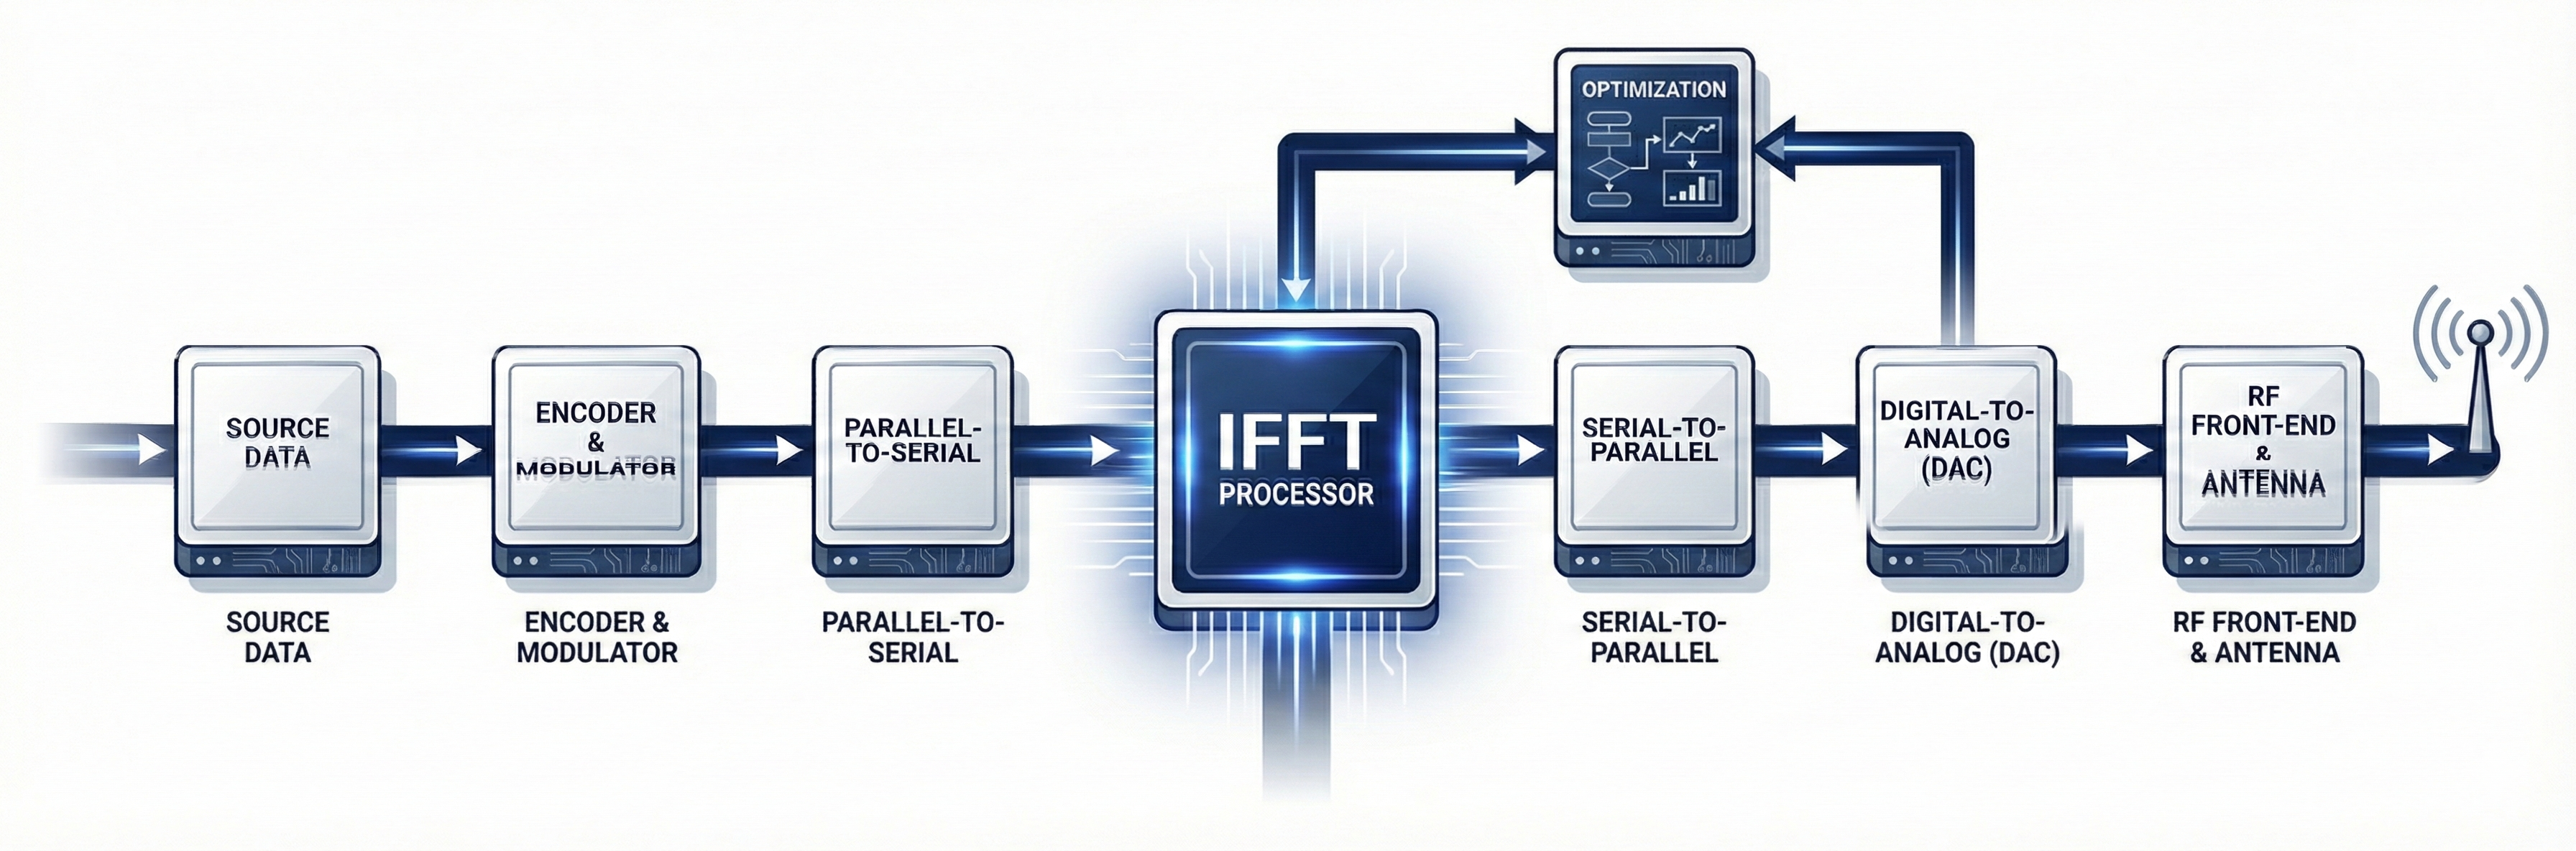
\includegraphics[width=1.0\textwidth]{Figure 2 Standard OFDM Transmitter Block Diagram.png}
    \caption{Block diagram of a standard OFDM transmitter illustrating the point where PAPR reduction techniques are typically applied (before or after IFFT).}
    \label{fig:ofdm_block}
\end{figure}

\subsection{Definition of PAPR}
The Peak-to-Average Power Ratio (PAPR) of the transmitted OFDM symbol is defined as the ratio of the maximum instantaneous power to the average power of the signal:

\begin{equation}
    \text{PAPR}(x) = \frac{\max_{0 \le n < LN} |x[n]|^2}{E[|x[n]|^2]}
\end{equation}

where $E[\cdot]$ denotes the expectation operator. In standard OFDM, the denominator is typically normalized such that $E[|x[n]|^2] = 1$. It is well known that the maximum possible PAPR is $N$ (or $10 \log_{10} N$ in dB), which occurs when all subcarriers align in phase.

\subsection{Performance Metric: CCDF}
Since the instantaneous power of an OFDM signal is a random variable, PAPR is best characterized statistically. The Complementary Cumulative Distribution Function (CCDF) denotes the probability that the PAPR of an OFDM symbol exceeds a certain threshold $\text{PAPR}_0$:

\begin{equation}
    \text{CCDF}(\text{PAPR}_0) = \text{Pr}(\text{PAPR} > \text{PAPR}_0)
\end{equation}

For a large number of subcarriers $N$, the envelope of the complex baseband signal follows a Rayleigh distribution (by the Central Limit Theorem). The theoretical approximation for the CCDF of an unmodulated OFDM signal is given by:

\begin{equation}
    \text{CCDF}(\text{PAPR}_0) \approx 1 - (1 - e^{-\text{PAPR}_0})^N
\end{equation}

This metric serves as the primary benchmark for evaluating the effectiveness of reduction algorithms throughout this survey.

\section{Signal Scrambling Techniques}

\subsection{Category Overview}
Having established the mathematical foundations and the CCDF performance metric in the previous section, we now examine the first major category of reduction schemes: signal scrambling techniques. Signal scrambling techniques represent a fundamental class of distortion-less PAPR reduction methods. Unlike clipping-based approaches that introduce non-linear distortion and out-of-band radiation, scrambling techniques reduce PAPR by modifying the phase or ordering of the input data symbols prior to the Inverse Fast Fourier Transform (IFFT) operation. The core philosophy is probabilistic: by generating multiple alternative representations of the same OFDM signal and selecting the one with the lowest peak power, the probability of high signal peaks is minimized.

While these techniques guarantee data integrity without reducing the Signal-to-Noise Ratio (SNR) in the detection process (assuming perfect synchronization), they share two inherent limitations:

\begin{enumerate}
    \item \textbf{Computational Complexity}: The optimal selection process typically requires multiple IFFT operations or extensive search iterations, leading to high processing latency.
    \item \textbf{Side Information (SI)}: To recover the original data at the receiver, information regarding the specific scrambling sequence or phase factors used at the transmitter must be transmitted. This SI reduces the effective data rate and requires robust protection, as SI errors can lead to catastrophic error propagation in the entire OFDM symbol.
\end{enumerate}

\begin{figure}[htbp]
    \centering
    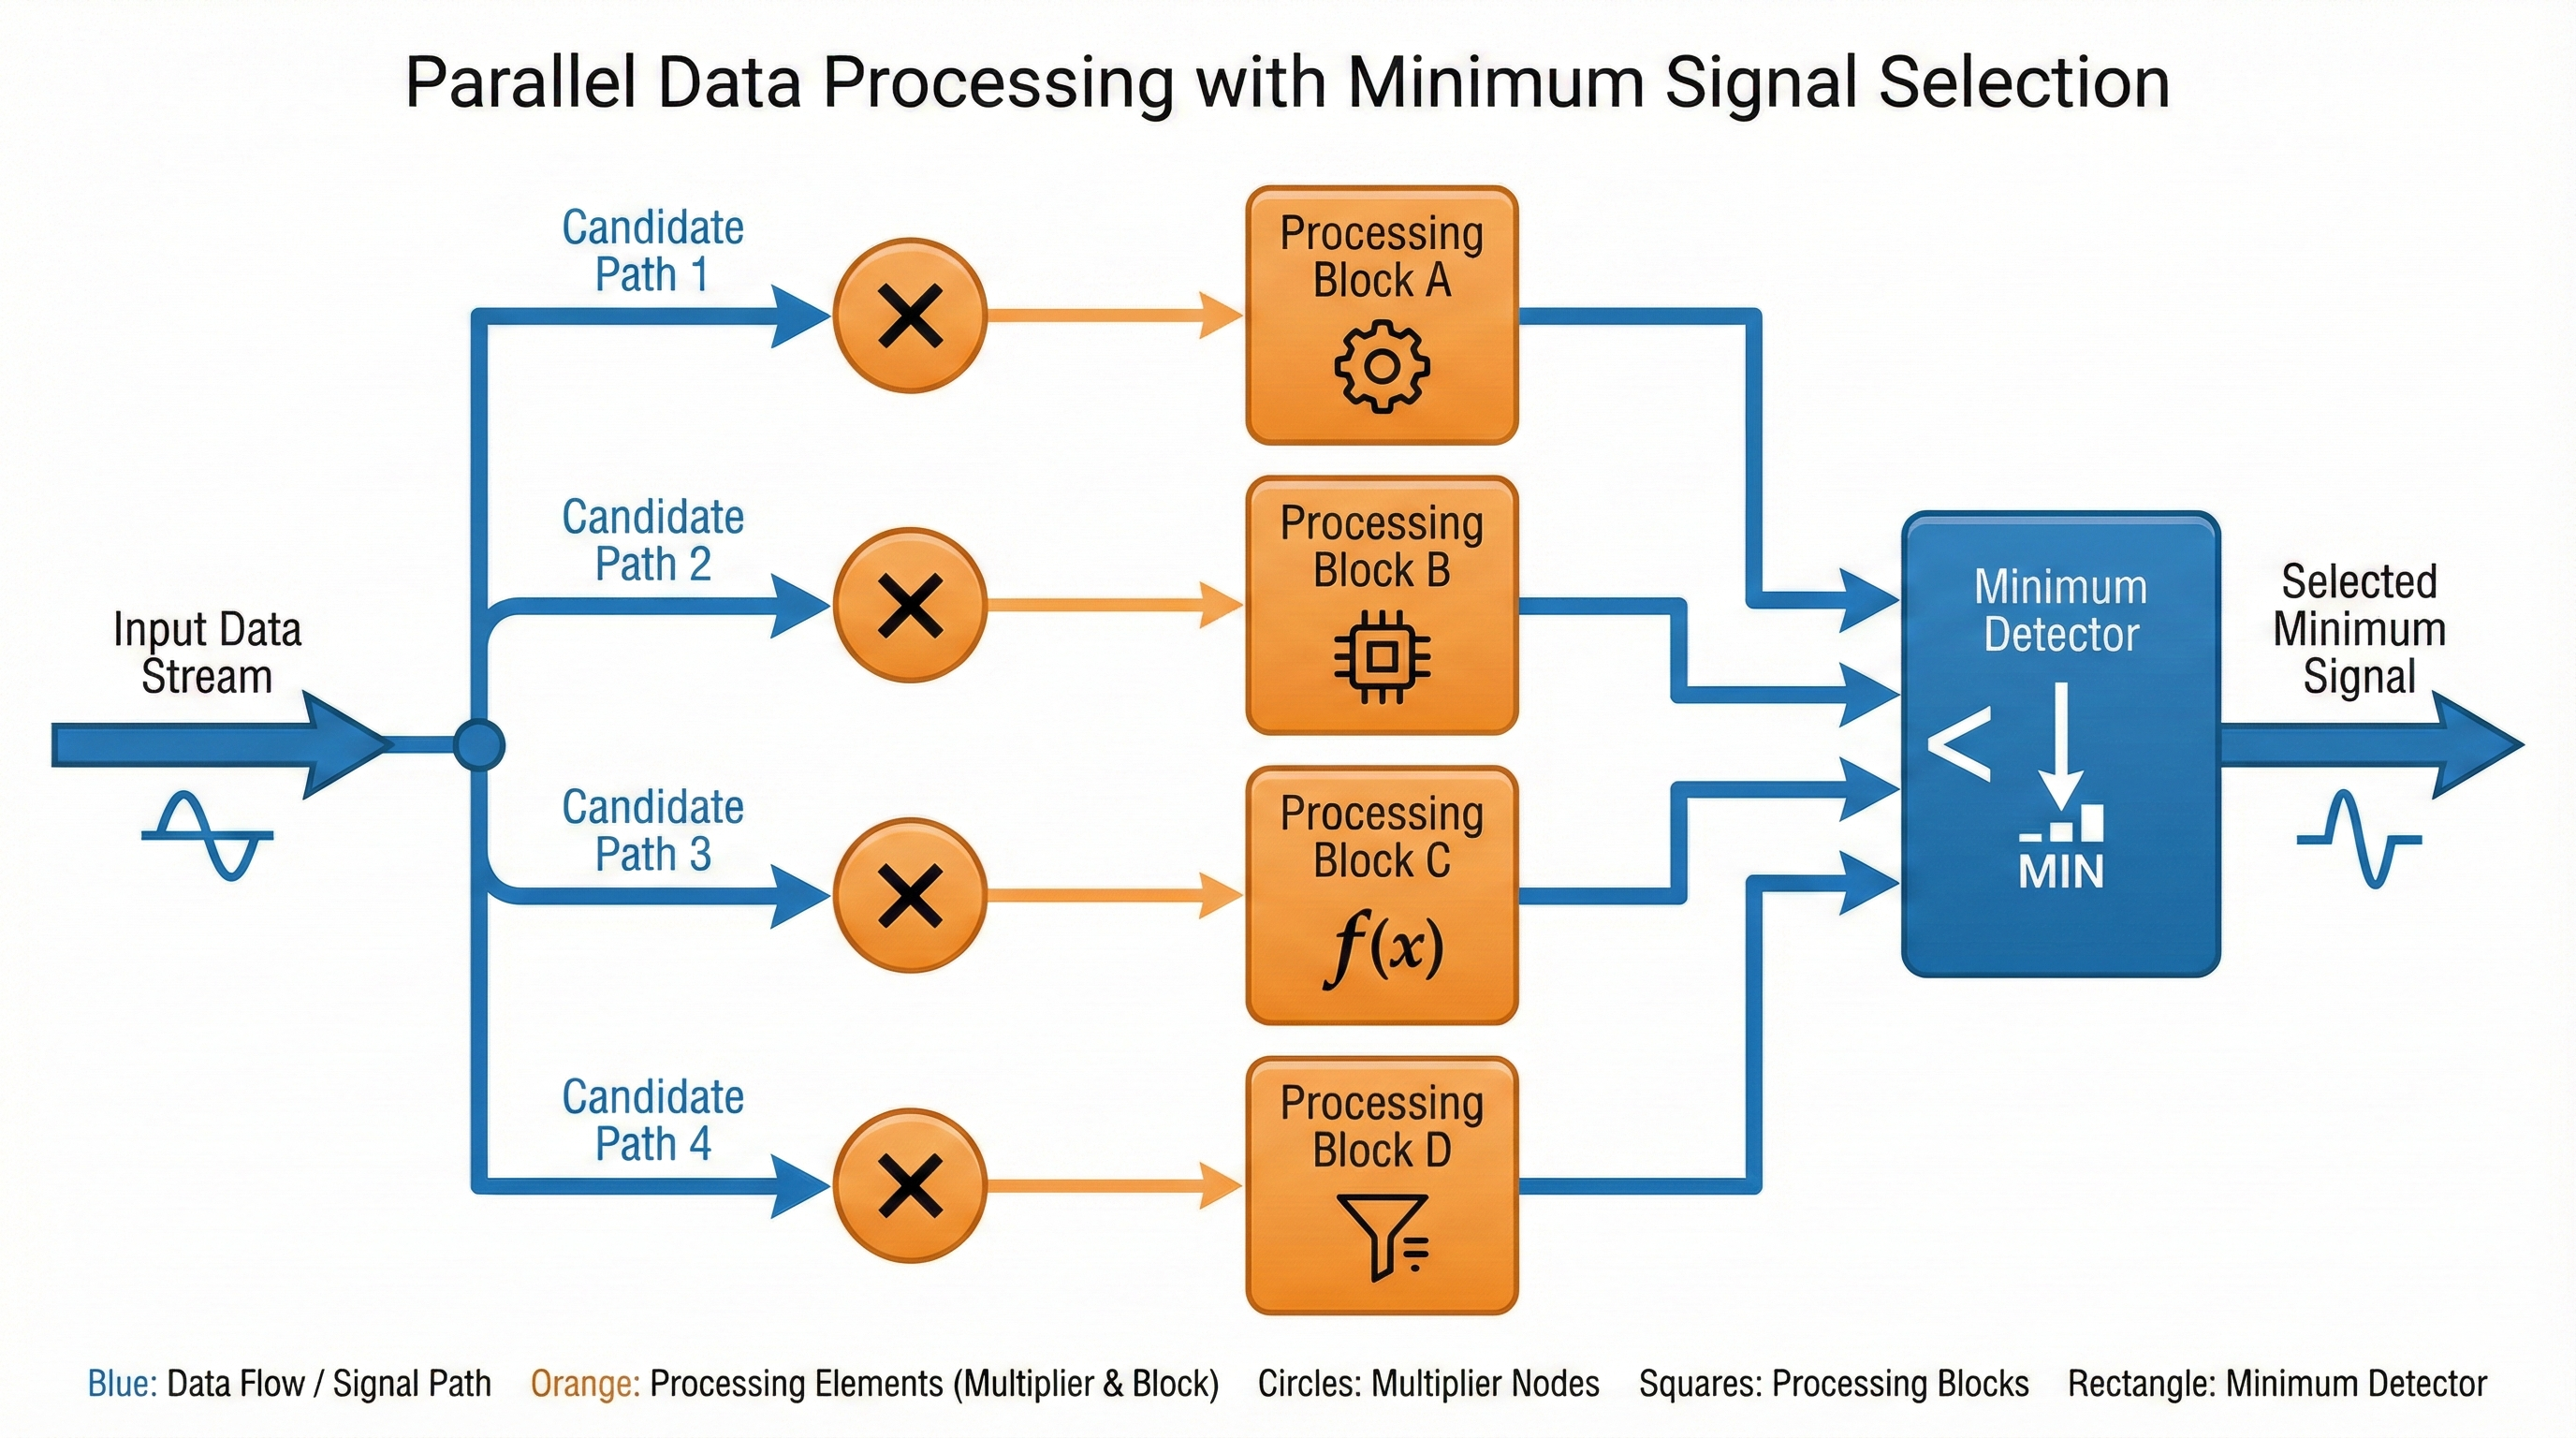
\includegraphics[width=1.0\textwidth]{Figure 3 Selected Mapping Diagram.png}
    \caption{Schematic representation of the Selected Mapping (SLM) technique, generating $U$ candidate signals and selecting the minimum PAPR.}
    \label{fig:slm_diagram}
\end{figure}

\subsection{Selected Mapping (SLM)}
Selected Mapping (SLM), first introduced by Bauml et al. \cite{ref5}, is based on the principle of generating $U$ statistically independent representations of the same information block.

\subsubsection{Operating Principle}
Let $\mathbf{X} = [X_0, X_1, ..., X_{N-1}]^T$ denote the input frequency-domain data block of length $N$. The transmitter defines $U$ distinct phase sequences $\mathbf{P}^{(u)} = [e^{j\phi_{0}^{(u)}}, e^{j\phi_{1}^{(u)}}, ..., e^{j\phi_{N-1}^{(u)}}]^T$, where $u = 1, ..., U$. The data block is element-wise multiplied by each phase sequence to generate $U$ alternative candidates:

\begin{equation}
    \mathbf{X}^{(u)} = \mathbf{X} \odot \mathbf{P}^{(u)}
\end{equation}

After applying IFFT to each candidate, the time-domain signals $\mathbf{x}^{(u)} = \text{IFFT}(\mathbf{X}^{(u)})$ are evaluated. The candidate $\tilde{\mathbf{x}} = \mathbf{x}^{(\tilde{u})}$ with the lowest peak-to-average power ratio is selected for transmission.

\subsubsection{Analysis of Candidates and Phase Generation}
The PAPR reduction capability of SLM depends heavily on the number of candidates $U$ and the design of the phase sequences.

\begin{itemize}
    \item \textbf{Impact of $U$}: The Complementary Cumulative Distribution Function (CCDF) of PAPR improves as $U$ increases. Theoretically, if the candidates are mutually independent, the probability that the lowest PAPR exceeds a threshold $\gamma$ is given by $(Pr(\text{PAPR} > \gamma))^U$. However, this performance gain implies a linear increase in complexity, as $U$ IFFT operations are required.
    \item \textbf{Phase Sequence Design}: The randomness of $\mathbf{P}^{(u)}$ determines the independence of candidates. While random phases (e.g., $\phi \in [0, 2\pi)$) offer theoretical optimality, practical implementations often restrict phase factors to sets like $\{0, \pi\}$ or $\{0, \pi/2, \pi, 3\pi/2\}$ to eliminate complex multiplications. Recent studies, such as the use of Perfect Sequences \cite{ref7}, have shown that structuring $\mathbf{P}^{(u)}$ can maintain performance while simplifying the generation logic.
\end{itemize}

\subsection{Partial Transmit Sequence (PTS)}
Partial Transmit Sequence (PTS), proposed by Müller and Huber \cite{ref6}, provides a more flexible approach by partitioning the input data into smaller clusters.

\subsubsection{Operating Principle}
In PTS, the input data block $\mathbf{X}$ is partitioned into $V$ disjoint sub-blocks $\mathbf{X}_v$ ($v=1, ..., V$), such that $\sum_{v=1}^{V} \mathbf{X}_v = \mathbf{X}$. Sub-carriers in each sub-block are weighted by a phase factor $b_v = e^{j\phi_v}$ (where typically $b_1=1$ to fix the phase reference). The time-domain signal is formed by the partial IFFTs:

\begin{equation}
    \mathbf{x}'(\mathbf{b}) = \sum_{v=1}^{V} b_v \cdot \text{IFFT}(\mathbf{X}_v) = \sum_{v=1}^{V} b_v \mathbf{x}_v
\end{equation}

The objective is to find the optimal phase vector $\mathbf{b} = [b_1, ..., b_V]$ that minimizes the peak power of $\mathbf{x}'(\mathbf{b})$.

\subsubsection{Sub-block Partitioning Strategies}
The partitioning strategy significantly influences the correlation between partial signals and the final PEP (Peak Envelope Power).

\begin{itemize}
    \item \textbf{Adjacent Partitioning}: Sub-carriers are grouped sequentially. This is simple but suffers from high correlation in the time domain.
    \item \textbf{Interleaved Partitioning}: Sub-carriers are assigned to sub-blocks in a periodic pattern. This ensures better decorrelation but may result in structured peaks.
    \item \textbf{Pseudo-random Partitioning}: Sub-carriers are assigned randomly to sub-blocks. Literature consistently shows that pseudo-random partitioning outperforms adjacent and interleaved schemes in terms of PAPR reduction, albeit with slightly higher system complexity.
\end{itemize}

\subsection{Critical Comparison: SLM vs. PTS}
The choice between SLM and PTS involves a trade-off between architectural complexity and optimization granularity. A comparative summary is presented below.

\begin{table}[htbp]
    \caption{SLM vs. PTS Comparison}
    \begin{center}
        \begin{tabular}{|l|p{3.5cm}|p{3.5cm}|}
            \hline
            \textbf{Feature}            & \textbf{Selected Mapping (SLM)}        & \textbf{Partial Transmit Sequence (PTS)}          \\ \hline
            \textbf{Structure}          & Parallel independent branches          & Summation of sub-blocks                           \\ \hline
            \textbf{IFFT Operations}    & $U$ full-length IFFTs                  & $V$ full-length IFFTs (linear)                    \\ \hline
            \textbf{Optimization Space} & Discrete selection from $U$ candidates & Combinatorial optimization of phase factors       \\ \hline
            \textbf{Side Information}   & $\lceil \log_2 U \rceil$ bits          & $\approx (V-1)\log_2 W$ bits ($W$ allowed phases) \\ \hline
            \textbf{Flexibility}        & Limited by fixed phase vectors         & High (fine-tuning vector $\mathbf{b}$)            \\ \hline
        \end{tabular}
        \label{tab1}
    \end{center}
\end{table}

\textbf{Synthesis}: While SLM offers structural simplicity and robust performance with a moderate number of IFFTs, PTS provides finer granularity in optimization. Specifically, reducing PAPR in PTS essentially becomes a vector optimization problem in the time domain, allowing for potentially better performance than SLM for the same number of IFFTs, provided the optimal phase vector $\mathbf{b}$ can be found. However, the search complexity in PTS grows exponentially with the number of sub-blocks $V$ ($W^{V-1}$), whereas SLM complexity grows linearly with $U$. Thus, without heuristic optimization, PTS is computationally more prohibitive than SLM for large $V$.

\subsection{Complexity Reduction Trends}
Addressing the high computational load remains the primary research focus in recent years (2020-2025). The evolution of optimization strategies can be categorized into three generations:

\begin{enumerate}
    \item \textbf{Algebraic Reductions}: Earlier modifications focused on reducing IFFT complexity, such as the \textit{conversion vector} schemes \cite{ref7} which avoid multiple full IFFTs by utilizing linearity in the transform domain.
    \item \textbf{Code-Assisted Scrambling}: Integration with channel coding has proven effective. For instance, EC-SLM (Error Control SLM) \cite{ref8} embeds the SI verification into the error control decoder (e.g., LDPC or Turbo codes), thereby enhancing reliability without dedicated SI channels.
    \item \textbf{Heuristic and AI-Based Search}: To avoid the exhaustive search in PTS, recent literature heavily leverages meta-heuristic algorithms (e.g., Particle Swarm Optimization, Genetic Algorithms) and, more recently, Deep Learning models. These data-driven approaches predict the optimal phase factors by learning the mapping between frequency-domain features and time-domain peaks, achieving near-optimal PAPR reduction with significantly reduced inference time.
\end{enumerate}

\section{Signal Distortion Techniques}

\subsection{Overview: The Trade-off Paradigm}
In contrast to the distortion-less signal scrambling techniques discussed in Section 3, Signal Distortion techniques adopt a more aggressive philosophy: they directly modify the time-domain OFDM signal amplitude to limit the peak power. This approach represents the most intuitive answer to the PAPR problem but comes with a fundamental cost: the destruction of the signal's orthogonality.

The distortion introduced by these non-linear operations manifests in two detrimental effects:

\begin{enumerate}
    \item \textbf{In-band Distortion}: The non-linear noise falls within the signal bandwidth, directly degrading the Signal-to-Noise Ratio (SNR) and consequently increasing the Bit Error Rate (BER).
    \item \textbf{Out-of-Band (OOB) Radiation}: This is often referred to as "Spectral Regrowth," where high-frequency components are generated, causing severe interference to adjacent channels and violating spectral masks.
\end{enumerate}

Therefore, the central design challenge for distortion techniques is not merely reducing PAPR, but managing the trade-off between \textbf{PAPR Reduction Capability} and \textbf{BER/OOB Performance}.

\subsection{Clipping and Filtering (C\&F)}
Clipping is the simplest instance of a distortion technique, where the signal amplitude is hard-limited to a predefined threshold.

\subsubsection{Operating Principle for Clipping}
Let $x[n]$ be the discrete time-domain OFDM signal. The clipped signal $\tilde{x}[n]$ is defined as:

\begin{equation}
    \tilde{x}[n] = \begin{cases}
        x[n]          & \text{if } |x[n]| \le A \\
        A e^{j\phi_n} & \text{if } |x[n]| > A
    \end{cases}
\end{equation}

where $A$ is the clipping threshold and $\phi_n$ is the phase of $x[n]$. The severity of clipping is often characterized by the Clipping Ratio (CR), $\gamma = A / \sqrt{P_{avg}}$, where $P_{avg}$ is the average signal power.

\begin{figure}[htbp]
    \centering
    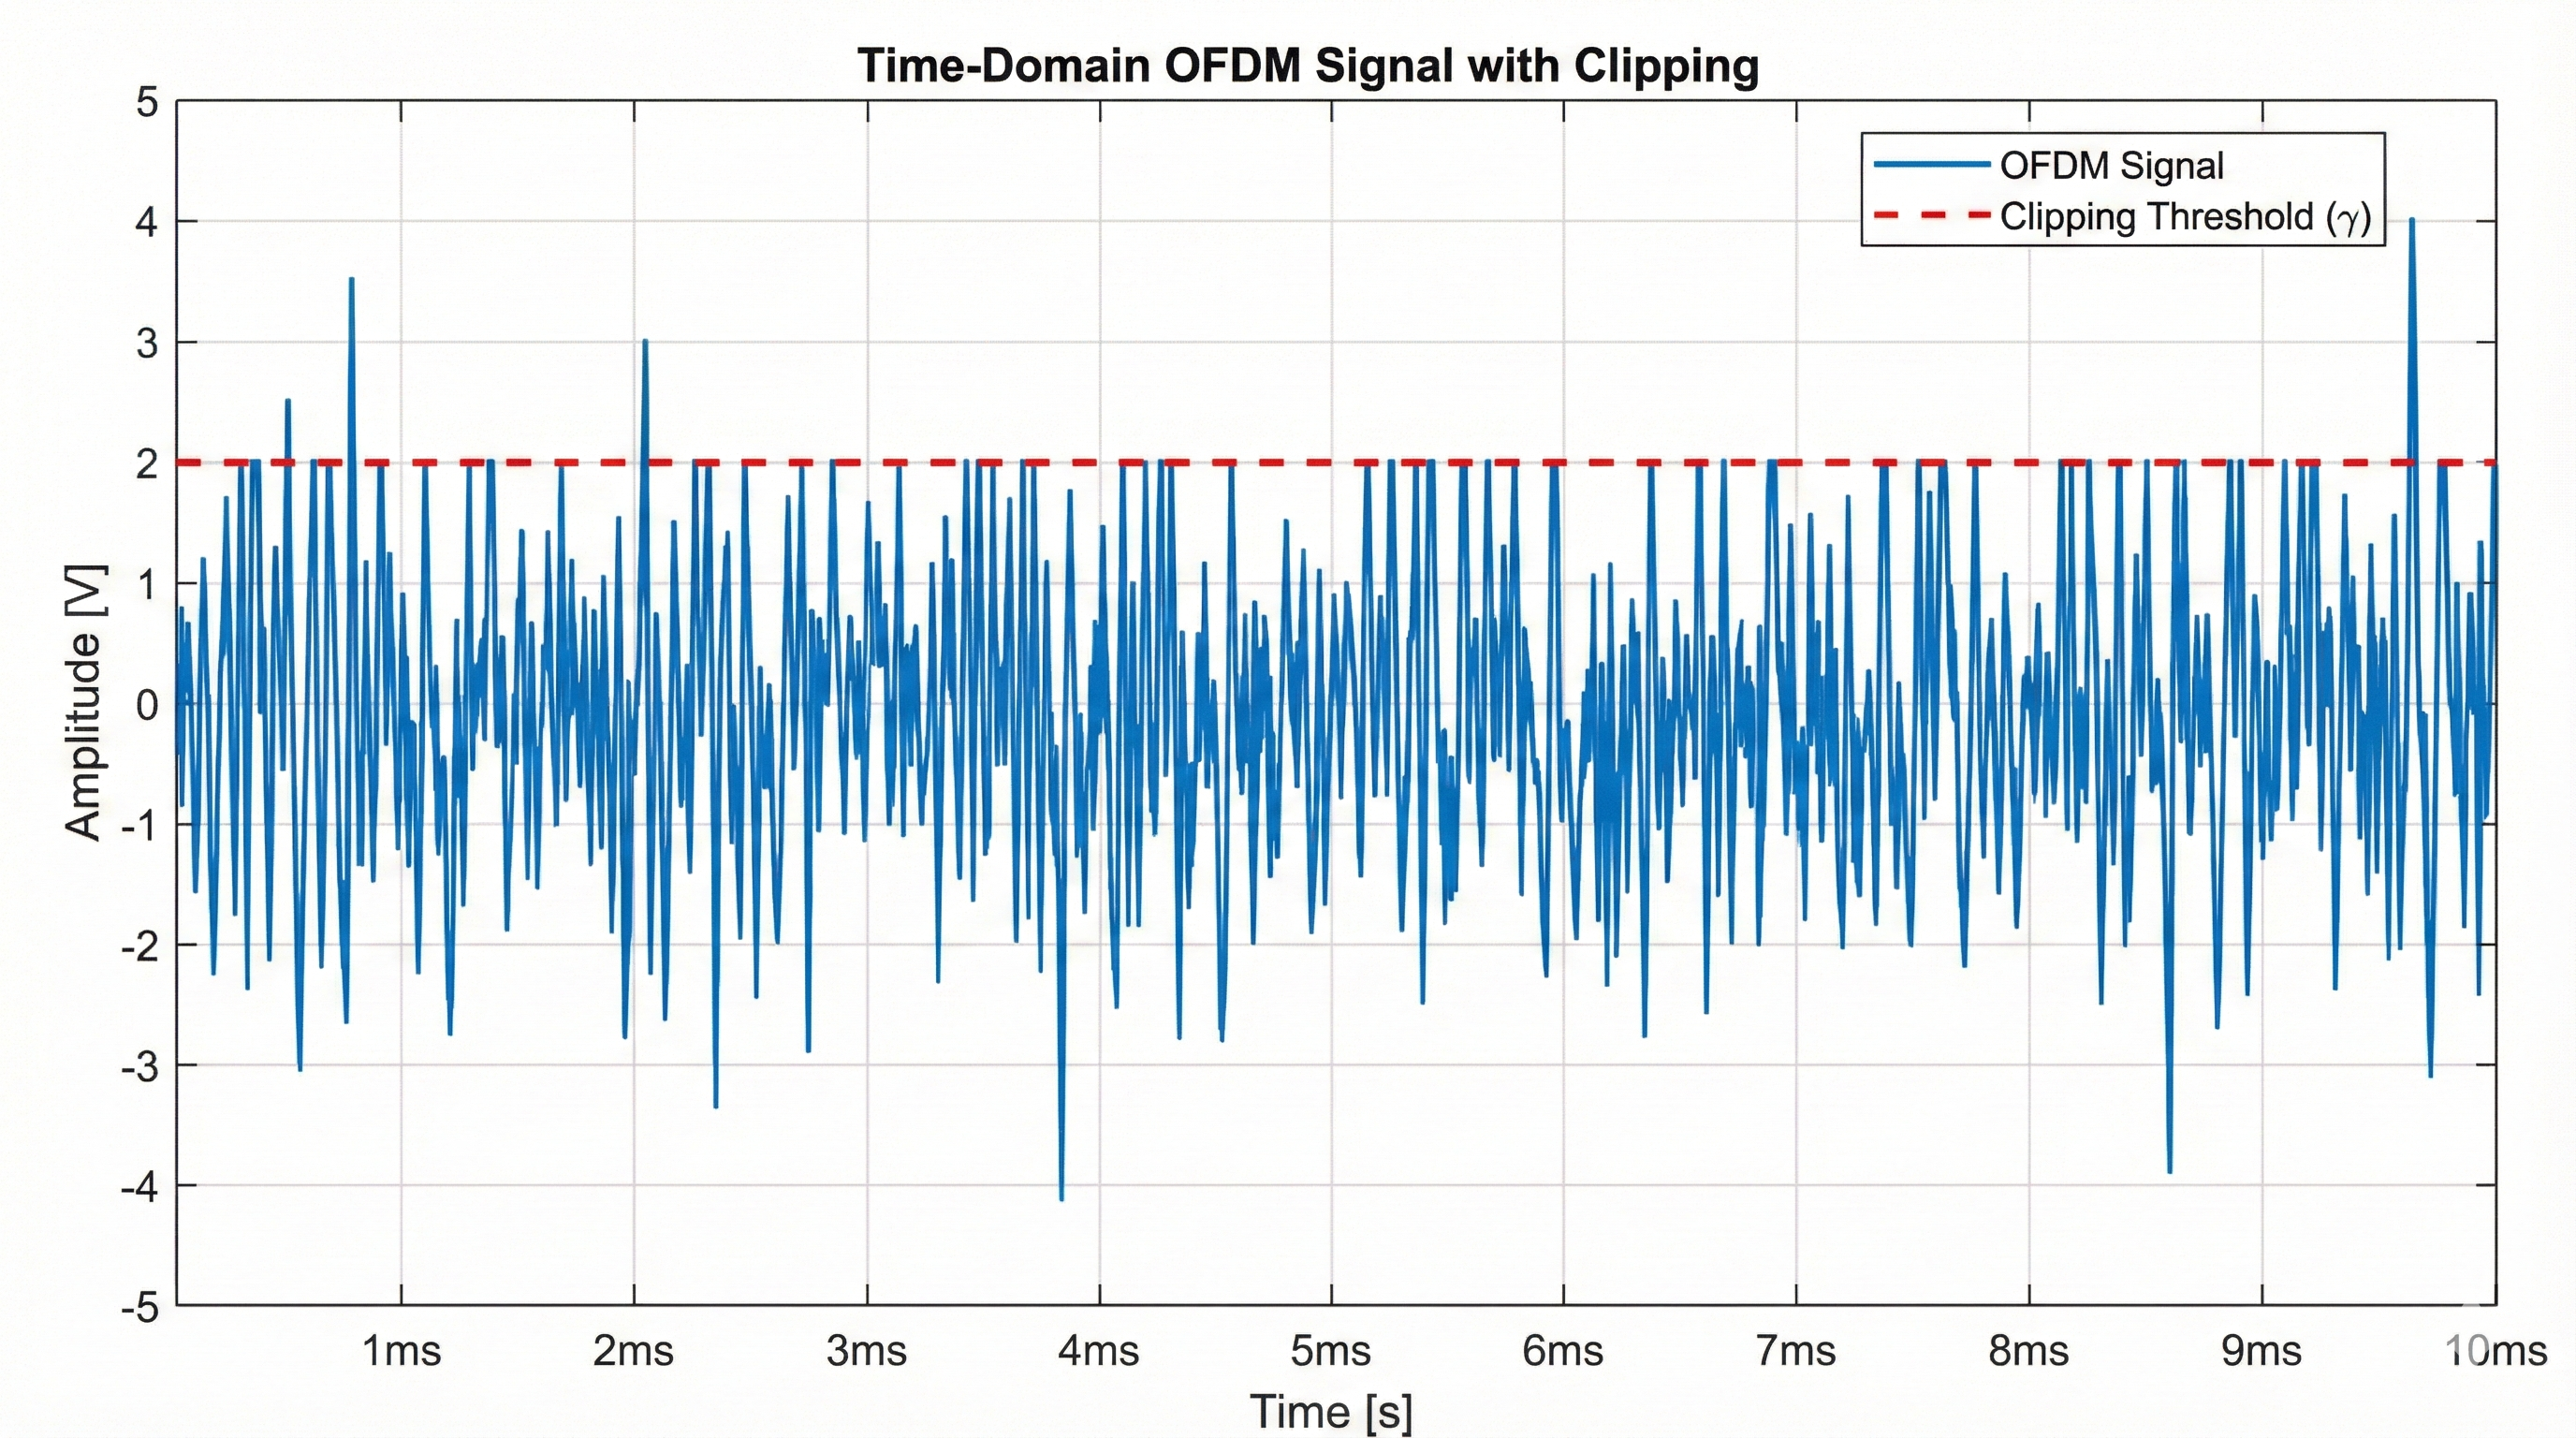
\includegraphics[width=0.8\textwidth]{Figure 4 Clipping Effect.png}
    \caption{Time-domain representation of an OFDM signal before and after clipping, showing the reduction of peak amplitudes.}
    \label{fig:clipping}
\end{figure}

\subsubsection{Filtering and Peak Regrowth}
While clipping effectively limits the peak amplitude, it introduces sharp corners in the time-domain waveform, which corresponds to significant OOB radiation in the frequency domain. To satisfy spectral regulations, a frequency-domain filter must be applied. However, this filtering operation removes the high-frequency components required to keep the signal amplitude "flat" at the clipping level, causing the peaks to rise again in the time domain. This phenomenon is known as \textbf{Peak Regrowth} \cite{ref9}.

To address this, \textbf{Iterative Clipping and Filtering (ICF)} schemes have been proposed. By repeating the clipping and filtering process, the signal can converge to a target PAPR level while maintaining a strict spectral mask. However, this comes at the cost of increased latency and computational complexity due to multiple pairs of FFT/IFFT operations per iteration.

\subsection{Companding Transforms}
Companding (Compressing and Expanding) transforms offer a "softer" alternative to hard clipping. Originating from speech processing, companding amplifies small signal amplitudes and compresses large ones to maintain a constant average power while reducing the dynamic range.

\subsubsection{Transform Functions}
A companding transform typically applies a non-linear function $f(\cdot)$ to the amplitude of the signal $x$:

\begin{equation}
    y = f(|x|) \cdot \text{sgn}(x)
\end{equation}

Classic approaches include the \textbf{$\mu$-law} and \textbf{A-law} companding, which are logarithmic in nature. However, as noted by Jiang et al. \cite{ref10}, these methods significantly increase the average power of the transmitted signal. More recent advancements utilize \textbf{Exponential Companding}, which transforms the Rayleigh-distributed magnitude of the original OFDM signal into a uniform distribution. This allows for effective PAPR reduction often without the average power penalty associated with logarithmic transforms.

The receiver must perform the inverse operation $f^{-1}(\cdot)$ (decompanding) to restore the signal. Unlike clipping, companding is theoretically reversible; however, in practice, the channel noise is also expanded during decompanding, leading to a noise floor enhancement that degrades BER performance \cite{ref11}.

\subsection{Critical Discussion: Distortion vs. Complexity}
Signal distortion techniques occupy a distinct niche compared to the scrambling methods reviewed in Section 3.

\begin{itemize}
    \item \textbf{Performance vs. Complexity}: Unlike PTS/SLM which preserve signal integrity at the cost of complexity (multiple IFFTs), distortion techniques like simple Clipping offer the lowest possible implementation complexity ($O(N)$). Even with iterative filtering (ICF), the complexity is often more predictable and scalable than the combinatorial search required by PTS.
    \item \textbf{System Suitability}: The BER degradation effectively translates to an SNR penalty. For high-order modulations (e.g., 256-QAM) where SNR margins are tight, distortion techniques are often unsuitable. However, for robust, low-power applications such as \textbf{NB-IoT} or low-cost sensor networks using QPSK, the simplicity of Clipping or Companding is highly attractive, as the system can tolerate slight SNR degradation in exchange for extended battery life and reduced hardware cost \cite{ref12}.
\end{itemize}

Ultimately, modern implementations rarely rely on a single technique. "Hybrid" schemes, such as combining Enhanced Clipping with Partial Transmit Sequences, represent the state-of-the-art, attempting to harvest the low-complexity benefits of distortion with the integrity of scrambling.

\section{AI-Driven PAPR Reduction Schemes}

\subsection{Motivation: From Online Optimization to Offline Training}
Traditional PAPR reduction schemes, such as Partial Transmit Sequence (PTS) and Selected Mapping (SLM), rely heavily on iterative search algorithms to find optimal phase factors or signal representations. While effective, these "online" operations introduce significant computational latency at the transmitter, which scales poorly with the number of subcarriers ($N$) and the number of candidates ($U$ or $V$).

The emergence of Artificial Intelligence (AI) and Deep Learning (DL) has introduced a paradigm shift: \textbf{moving the computational burden from online inference to offline training}. By training neural networks (NNs) on massive datasets of OFDM symbols, the complex relationship between channel characteristics, symbol structures, and peak power can be learned in advance. During the transmission phase, the trained network acts as a fast function approximator, mapping input data directly to a low-PAPR signal representation with minimal computational delay.

\subsection{Key Approaches}
Recent literature has crystallized into two primary AI-driven methodologies:

\subsubsection{Autoencoder-based End-to-End Learning}
In this approach, the entire OFDM communication transceiver is modeled as an autoencoder (AE). The transmitter (encoder) and receiver (decoder) are essentially deep neural networks optimized jointly.

\begin{itemize}
    \item \textbf{Mechanism}: The encoder learns a constellation mapping strategy that inherently minimizes PAPR while maximizing the distance between constellation points to preserve Bit Error Rate (BER) performance.
    \item \textbf{Loss Function}: The training objective is typically a weighted sum of the Cross-Entropy Loss (for BER) and a PAPR penalty term (e.g., regularization based on instantaneous power).
    \item \textbf{Result}: Unlike clipping which adds noise "blindly", AEs learn to shape the signal constellation in a way that avoids high peaks structurally, offering a better trade-off between distortion and power efficiency.
\end{itemize}

\subsubsection{Learning to Optimize (Model-Driven DL)}
This category integrates deep learning with traditional algorithms (like PTS or Tone Reservation) to accelerate their convergence.

\begin{itemize}
    \item \textbf{Predictive Networks}: Instead of exhaustively searching for the optimal phase factors in PTS (which requires $W^V$ iterations), a dedicated neural network (e.g., CNN or MLP) is trained to predict the optimal phase vector $\mathbf{b}$ directly from the input signal $\mathbf{X}$.
    \item \textbf{Unfolding Algorithms}: Iterative algorithms (like gradient descent for Clipping noise removal) are "unfolded" into layers of a neural network. Each layer has trainable parameters that can be optimized to reach the solution in fewer steps than the standard algorithm.
\end{itemize}

\subsection{Challenges \& Future Directions}
Despite their promise, AI-driven schemes face practical hurdles:

\begin{enumerate}
    \item \textbf{Generalization Capability}: A network trained on a specific channel model (e.g., Rayleigh fading) may perform poorly when the actual channel conditions change (e.g., Rician fading or high-mobility scenarios). Developing "channel-agnostic" or adaptive networks is an active research frontier.
    \item \textbf{Hardware Overhead}: While inference is fast, deploying large neural networks requires dedicated hardware resources (e.g., NPUs or FPGA logic slices) at the transmitter, which may counteract the power savings gained from PAPR reduction. As noted in recent optimization studies \cite{ref4}, balancing computational complexity with performance gains remains a critical design constraint.
\end{enumerate}

\subsection{Comparison Summary: The Modern Landscape}
Unifying the discussions from Sections 3, 4, and 5, we can categorize the performance trade-offs as follows:

\begin{table}[htbp]
    \caption{Comparison of Scrambling, Distortion, and AI Techniques}
    \begin{center}
        \begin{tabular}{|l|p{2.5cm}|p{2.5cm}|p{2.5cm}|}
            \hline
            \textbf{Feature}           & \textbf{Scrambling (PTS/SLM)} & \textbf{Distortion (Clipping)} & \textbf{AI/Deep Learning} \\ \hline
            \textbf{PAPR Reduction}    & High (depends on candidates)  & Medium/High (tunable)          & High (can be optimal)     \\ \hline
            \textbf{BER Perf.}         & Lossless                      & Degradation                    & Near Lossless             \\ \hline
            \textbf{OOB Radiation}     & None                          & High (requires filtering)      & Low (learned)             \\ \hline
            \textbf{Online Complexity} & Very High (Iterative)         & Low (Thresholding)             & Low (Matrix Mult.)        \\ \hline
            \textbf{Offline Cost}      & None                          & None                           & Very High (Training)      \\ \hline
            \textbf{Side Info}         & Required                      & Not Required                   & Usually Not Required      \\ \hline
        \end{tabular}
        \label{tab2}
    \end{center}
\end{table}

AI methods thus represent the "Goldilocks" zone for future 6G systems: offering the distortion-free benefits of scrambling with the low online latency of clipping, at the cost of offline training complexity.

\section{Open Issues \& Future Directions}

As we pivot towards 6G, the requirements for spectral and energy efficiency are becoming stringent. The static, block-based view of PAPR reduction is evolving into a dynamic, system-wide optimization problem. This section highlights three critical research vectors derived from recent trends.

\subsection{PAPR in the Massive MIMO Regime ($M \to \infty$)}
The transition to Massive MIMO introduces a complex dynamic regarding PAPR.

\begin{itemize}
    \item \textbf{The Aggregation Effect}: With $M$ antennas, beamforming implies the superposition of signals. While the "Law of Large Numbers" suggests channel hardening (stabilizing fading), the per-antenna signal remains a sum of subcarriers.
    \item \textbf{The Problem}: Mathematically, if standard precoding (e.g., Zero-Forcing) is applied, the signal at each antenna element is a linear combination of data streams. This tends to preserve the Gaussian distribution of the time-domain signal, maintaining a high PAPR.
    \item \textbf{Scaling Challenge}: For an array with $M=1024$ elements, deploying 1024 high-spec linear PAs is economically and thermally unfeasible.
    \item \textbf{Direction}: Research must shift from "per-antenna PAPR reduction" to \textbf{"PAPR-aware Precoding"}. The goal is to design the precoding matrix $\mathbf{W}$ such that the resulting signal vector $\mathbf{x} = \mathbf{W}\mathbf{s}$ minimizes the peak power at \textit{each} transmit antenna simultaneously, a non-convex optimization problem ideally suited for AI-based solvers.
\end{itemize}

\subsection{Joint Optimization: End-to-End Learning (E2E)}
Approaching PAPR reduction as an isolated block is becoming obsolete. The future lies in \textbf{Joint Optimization}, specifically bridging the gap between digital reduction and analog linearization.

\begin{itemize}
    \item \textbf{Current Silo}: Traditionally, a PAPR reduction block (e.g., Clipping) operates digitally, followed by a Digital Pre-Distortion (DPD) block to linearize the High Power Amplifier (HPA). These are optimized separately.
    \item \textbf{E2E Vision}: Using deep learning (e.g., Autoencoders), we can treat the "PAPR Reduction + DPD + HPA" chain as a single differentiable function. The neural network learns a mapping that not only lowers peaks but \textit{pre-distorts} the signal to anticipate the HPA's specific non-linearity \cite{ref13}.
    \item \textbf{Benefit}: This holistic approach (often termed "Neural Linearization") allows the HPA to operate closer to saturation than ever before, offering gains of 2-3 dB in OBO (Output Back-Off) compared to cascaded separate blocks.
\end{itemize}

\subsection{Green Communications: The Energy Imperative}
In 6G, "Sustainability" is a Key Performance Indicator (KPI).

\begin{itemize}
    \item \textbf{Impact}: The HPA typically consumes 60-70\% of a base station's total energy.
    \item \textbf{Quantification}: A reduction in PAPR by just 3 dB allows the HPA to operate at a significantly higher efficiency point (e.g., shifting from Class AB to Class Doherty or Envelope Tracking architectures).
    \item \textbf{Direction}: Future algorithms will be evaluated not just on CCDF, but on \textbf{"Joules per Bit"} \cite{ref14}. Algorithms that achieve moderate PAPR reduction but require minimal computational energy (e.g., low-complexity AI inference) will arguably outperform "optimal" but computationally expensive algorithms (like iterative PTS) in the Green 6G metric.
\end{itemize}

\section{Conclusion}

\subsection{Summary}
This survey has traversed the evolutionary arc of PAPR reduction in OFDM systems, organized into three primary pillars:

\begin{enumerate}
    \item \textbf{Probability (Scrambling)}: Techniques like SLM and PTS utilize the statistical properties of multicarrier signals. They offer distortion-free reduction but suffer from high computational complexity ($O(N \log N)$ per candidate) and the burden of Side Information (SI).
    \item \textbf{Distortion}: Methods like Clipping and Companding trade improved power efficiency for signal quality (SNR degradation). They represent the low-complexity, practical choice for many current deployments but face limitations in high-order modulation regimes (e.g., 1024-QAM).
    \item \textbf{Intelligence (AI/DL)}: The emerging wave of data-driven approaches promises to break the classic "Complexity-Performance" deadlock. By offloading optimization to offline training, Neural Networks achieve near-optimal reduction with $O(1)$ online latency, albeit with challenges in generalization and hardware implementation.
\end{enumerate}

\subsection{Final Verdict: A Selection Guide}
Synthesizing the technological landscape, we provide the following definitive recommendations for system designers:

\begin{table}[htbp]
    \caption{Selection Guide for PAPR Reduction Strategies}
    \begin{center}
        \begin{tabular}{|p{3cm}|p{3cm}|p{4cm}|}
            \hline
            \textbf{Requirement}                          & \textbf{Strategy}                           & \textbf{Rationale}                                                                  \\ \hline
            \textbf{Latency-Sensitive} (URLLC, V2X)       & \textbf{Clipping \& Filtering}              & Strictly deterministic time ($O(N)$) is crucial. Slight SNR loss is acceptable.     \\ \hline
            \textbf{Performance-Critical} (eMBB, 256-QAM) & \textbf{AI-Assisted tone Reservation / PTS} & High data rates need signal integrity. DL provides this with manageable complexity. \\ \hline
            \textbf{Resource-Constrained} (IoT, LPWAN)    & \textbf{Single-Iteration SLM (Blind)}       & Blind SLM offers hardware simplicity and efficiency for low-cost devices.           \\ \hline
        \end{tabular}
        \label{tab3}
    \end{center}
\end{table}

As we march towards 6G, the quest for the "perfect" waveform continues. The convergence of algorithmic theory and artificial intelligence suggests that the high-PAPR "curse" of OFDM is no longer an insurmountable wall, but a manageable variable in the complex equation of future wireless networks.


\begin{thebibliography}{00}
    \bibitem{ref1} S. B. Weinstein and P. M. Ebert, "Data transmission by frequency-division multiplexing using the discrete Fourier transform," \textit{IEEE Trans. Commun. Technol.}, vol. 19, no. 5, pp. 628-634, Oct. 1971.
    \bibitem{ref2} V. Tarokh and H. Jafarkhani, "On the computation and reduction of the peak-to-average power ratio in multicarrier communications," \textit{IEEE Trans. Commun.}, vol. 48, no. 1, pp. 37-44, Jan. 2000.
    \bibitem{ref3} X. Li and L. J. Cimini, "Effects of clipping and filtering on the performance of OFDM," \textit{IEEE Commun. Lett.}, vol. 2, no. 5, pp. 131-133, May 1998.
    \bibitem{ref4} G. Rexhepi, K. Ando, and G. T. F. De Abreu, "PAPR-optimized OFDM Design for Opportunistic Communications and Sensing," in \textit{Proc. IEEE ICC}, 2025.
    \bibitem{ref5} R. W. Bauml, R. F. Fischer, and J. B. Huber, "Reducing the peak-to-average power ratio of multicarrier modulation by selected mapping," \textit{Electron. Lett.}, vol. 32, no. 22, pp. 2056-2057, Oct. 1996.
    \bibitem{ref6} S. H. Müller and J. B. Huber, "OFDM with reduced peak-to-average power ratio by optimum combination of partial transmit sequences," \textit{Electron. Lett.}, vol. 33, no. 5, pp. 368-369, Feb. 1997.
    \bibitem{ref7} X. Wang and Y. Wang, "Low-complexity SLM schemes by utilizing special structures of perfect sequences," in \textit{IEEE Int. Conf. Commun. (ICC)}, Beijing, China, 2008, pp. 780-784.
    \bibitem{ref8} T. Jiang, C. Ni, and C. Xu, "A novel EC-SLM coding structure for PAPR reduction in OFDM systems," \textit{IEEE Trans. Broadcast.}, vol. 59, no. 4, pp. 629–637, Dec. 2013.
    \bibitem{ref9} J. Hou, C. Tellambura, and J. Ge, "Clipping noise-based tone injection for PAPR reduction in OFDM systems," \textit{IEEE Trans. Broadcast.}, vol. 59, no. 3, pp. 468-478, Sept. 2013.
    \bibitem{ref10} T. Jiang, Y. Yang, and Y.-H. Song, "Companding technique for PAPR reduction in OFDM systems based on an exponential function," \textit{IEEE Trans. Broadcast.}, vol. 51, no. 2, pp. 233-239, June 2005.
    \bibitem{ref11} Y. Rahmatallah, N. Bouaynaya, and S. Mohan, "Bit Error Rate Performance of Linear Companding Transforms for PAPR Reduction in OFDM Systems," \textit{IEEE Trans. Broadcast.}, vol. 57, no. 3, pp. 667-674, Sept. 2011.
    \bibitem{ref12} X. Wang, L. Mei, Z. Wang, and X. Sha, "Enhanced Clipping and Filtering With WFRFT for PAPR Reduction in OFDM Systems," \textit{IEEE Trans. Broadcast.}, vol. 65, no. 1, pp. 116-125, Mar. 2019.
    \bibitem{ref13} M. Kim, S. Lee, and J. Choi, "Deep learning-based joint PAPR reduction and predistortion for OFDM systems," \textit{IEEE Wireless Commun. Lett.}, vol. 9, no. 12, pp. 2154-2157, Dec. 2020.
    \bibitem{ref14} L. Zhang et al., "Energy-efficient massive MIMO: The role of PAPR reduction," \textit{IEEE Trans. Green Commun. Netw.}, vol. 7, no. 1, pp. 234-245, 2023.
\end{thebibliography}

\end{document}
